 \begin{frame}{Data description}
     \begin{itemize}[label=*]
        \item 
            we use the dataset of new symptomatic and 
            confirmed COVID-19 reported cases daily in Mexico City, considering 
            that its population is $N=26446435$.
        \item 
            The dataset contains 
            47 records in the period March 10 to April 25, 2020.
        \item  
            We use 
            these records $I^o_s$ to construct the observations, the process 
            $I_s:=I^o_s/N$.  
        \item  
            Combining $I_s$ and the Milstein scheme, we generate the
            others four processes of the system  with the parameters of Table
            \ref{table:parametermodel}, 
            $\sigma=1/100$ and $\Delta=1/1000$.
    \end{itemize}
\end{frame}
%------------------------------------------------------------------------------
\begin{frame}{Data construction }
    \begin{algorithm}[H]
        \caption{Construction of dataset.} \label{Alg-ds}  
        \begin{algorithmic}[1]
            \State Using initial conditions and make $n=0$.
            \State Generate 
                $\Delta W\sim N(0,\Delta)$.
            \State 
                $
                    S(t_{n+1}) = 
                        S(t_n) - (\mu+\beta_aI_a(t_{n}) 
                        + \beta_s I_s^{mx}(t_n))\Delta S(t_{n}) 
                        + (\mu+\gamma R(t_n)) * \Delta 
                        - \sigma(1-S(t_n))\Delta W
                $
            \State 
                $
                    E(t_{n+1}) = E(t_{n}) - (\kappa+\mu) * \Delta E(t_{n}) 
                    + \Delta * (\beta_sI_s ^ {mx}(t_n) 
                    + \beta_aI_a(t_{n})S(t_n)
                    - \sigma(E(t_n))\Delta W
                $
            \State 
                $
                    I_a(t_{n+1}) = I_a(t_{n}) 
                        - p\kappa E(t_{n}) \Delta I_a(t_{n})
                        - (\alpha_a+\mu)I_a(t_{n})\Delta
                        - \sigma I_a(t_{n})\Delta
                $
            \State 
                $
                    R(t_{n+1}) = 1 - S(t_{n+1}
                        - E(t_{n+1}) - I_a(t_{n+1})
                        - I^{mx}_s(t_{n+1})
                $.
            \State If $n<47$ make $n=n+1$ and go to 2. In other case stop.
        \end{algorithmic}
    \end{algorithm}
\end{frame}
%-------------------------------------------------------------------------------
%  \begin{frame}{Initial conditions}
% \begin{table}[tbh]
%         \centering
%         \begin{tabular}{
%             rl  
%         }
%             \hline
%             Process & Value
%             \\
%           \hline
            
%             $E(0)$ & 198.504525/N
                 
%             \\
%             $I_a(0)$ & 
%                 99.174034/N
%             \\
%             $I_s(0)$ & 74/N
                
%             \\
               
%             $R(0)$ & 
%                 0 
%             \\
%             $S(0)$ &  $1-(E(0)+I_a(0)+I_s(0)+R(0))$ 
%             \\      
        
%            \hline
%         \end{tabular}
%         \caption{Initial Conditions.}
%         \label{table:initial}
%     \end{table}
%     \end{frame}

\subsection{Estimation of parameters}
\begin{frame}{Estimators for real data}
    We assume the following parameters as given:
    $\gamma =1 /365$,
    $\kappa = 0.196078$,
    $\alpha_a = 0.167504$ 
    $\alpha_s = 0.092507$. 
    We generate 1000 datasets using the data of Mexico City. 
    \begin{table}[tbh]
        \centering
        \begin{tabular}{%w
                %>{\centering}
                %p{1in}
                %p{3in}
                %p{0.57\textwidth}
            rccc
        }
            \hline
            Parameter  & Estimator & CIL & CIU
            \\
              \hline
            
            $\beta_s$ 
            
            &  0.059159 & 0.002546&
            0.115772
            \\
            $\beta_a$ 
        
            & 0.509925 & 0.378248 &
            0.641603
            \\
        
            $p$ 
            
            &0.582808 &0.582326&0.583289
            \\          
            $\sigma$ & 1.31701E-002
            & 8.32156E-003&
            1.94434E-002\\
                  \hline
        \end{tabular}
        \caption{
            Average and  95\% confidence interval of the estimator of 
            $\sigma$ and MLEs for $\beta_a,\beta_s$, and $p$.
        }
        \label{table:MLEREAL}
    \end{table}
\end{frame}
%-------------------------------------------------------------------------------------------
\begin{frame}
    \begin{figure}[htb]
        \centering
        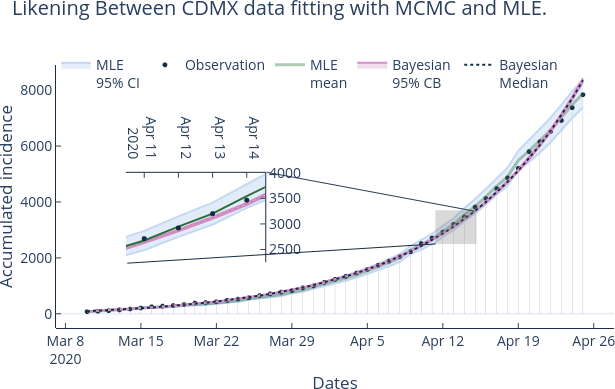
\includegraphics[width=1.0\textwidth, keepaspectratio]{assets/Likening.png}
     
        \label{fig:real_data_fitting}
    \end{figure}    
\end{frame}
%--------------------------------------------------------------------------------------------

\subsection{Validation of the model}
\begin{frame}{Validation of the model}
    \begin{figure}[htb]
        \centering
        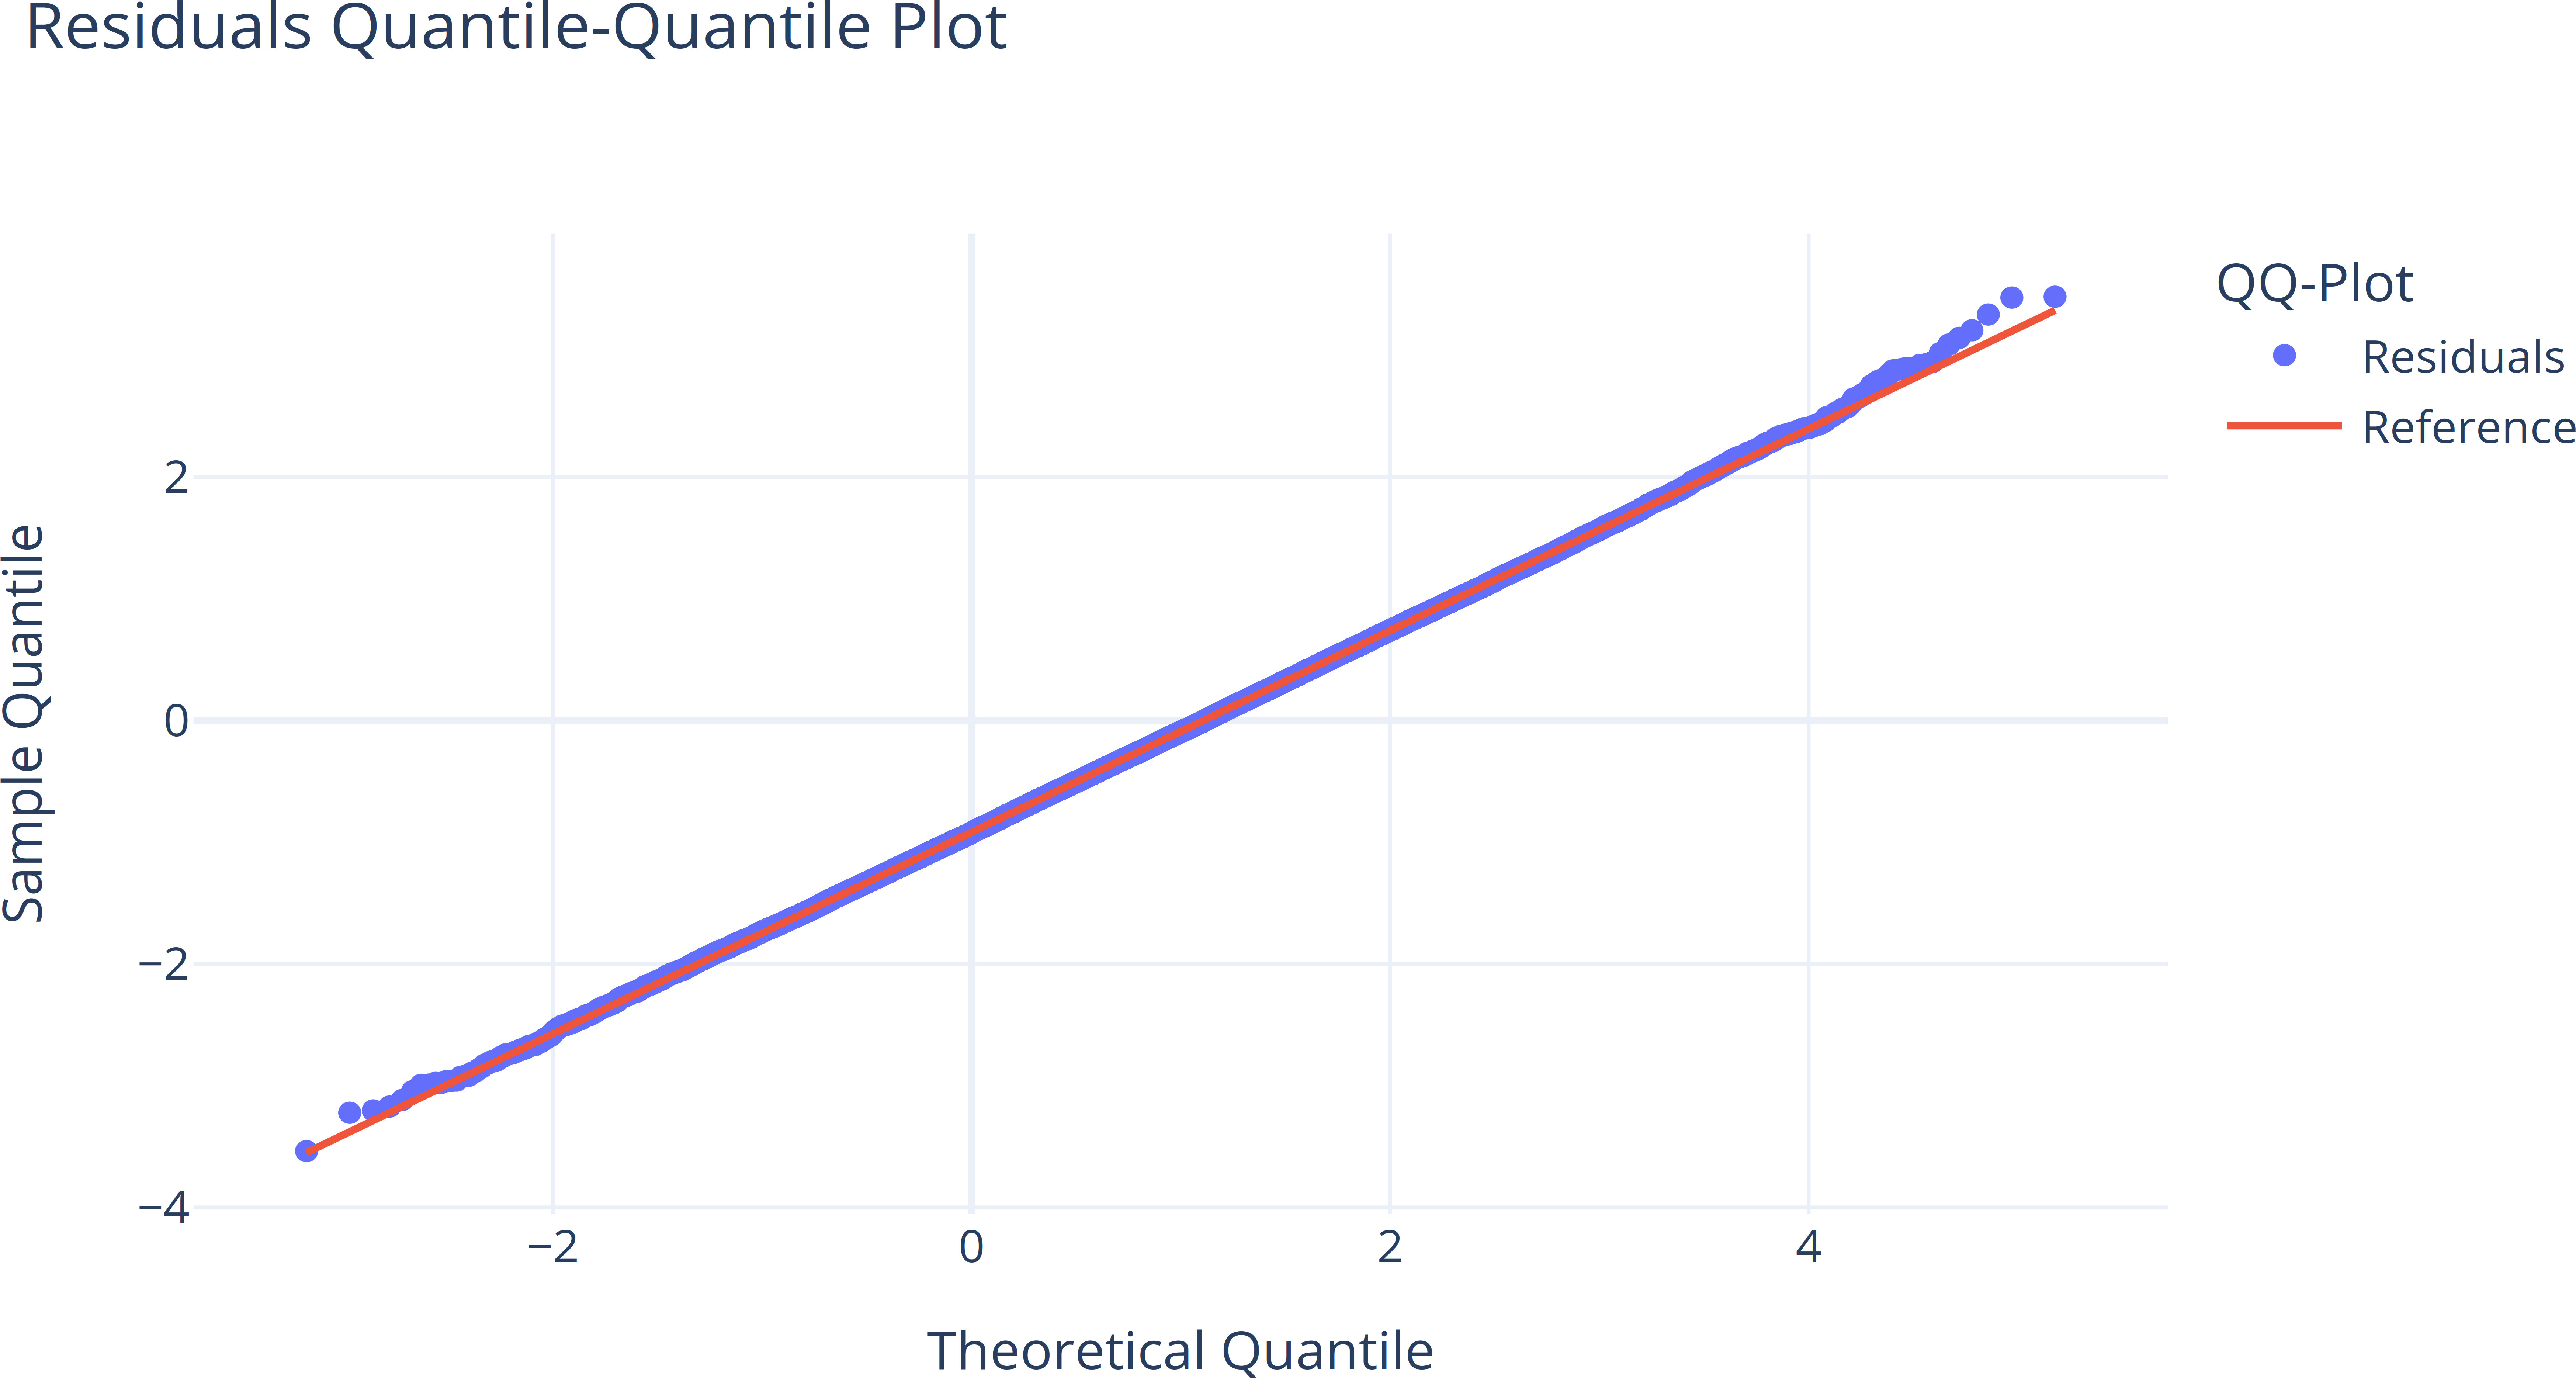
\includegraphics[scale=0.6]{assets/qq_plot.png}
        \caption{Quantile-Quantile plot of the numerical residuals.}
         \label{fig:fig_qq}
     \end{figure}
\end{frame}